\section{Visione Generale della Strategia di Verifica}

\subsection{Definizione obiettivi}

\subsubsection{Qualità di Processo}
Per garantire la qualità del prodotto è necessario perseguire la qualità dei processi che lo definiscono. Per fare questo si è deciso di adottare lo standard ISO /IEC$_G$ 15504 denominato SPICE il quale fornisce gli strumenti necessari a valutare l’idoneità di questi ultimi. Per applicare correttamente questo modello si deve utilizzare il ciclo di Deming (ciclo PDCA) il quale definisce una metodologia di controllo dei processi durante il loro ciclo di vita che consente di migliorarne in modo continuativo la qualità.

\subsubsection{Qualità di Prodotto}
Al fine di aumentare il valore commerciale di un prodotto software e di garantirne il corretto funzionamento è necessario fissare degli obiettivi qualitativi e di garantire che questi vengano effettivamente rispettati. Lo standard ISO/IEC$_G$ 91264 è stato redatto con lo scopo di descrivere questi obiettivi e delineare delle metriche capaci di misurare il raggiungimento di tali obiettivi.

\subsection{Controllo di qualità}

\subsubsection{Procedure di controllo di qualità di processo}
La qualità dei processi viene monitorata mediante l'analisi costante della qualità del prodotto. Un prodotto di bassa qualità è indice di carenza di qualità anche nei processi coinvolti alla realizzazione di quel prodotto, e quindi indica un processo da migliorare. Per quantificare la qualità dei processi il team si impegna ad utilizzare le metriche descritte nella sezione 3.7.3.
\\
Per avere controllo dei processi, e conseguentemente qualità, è necessario che:
\begin{itemize}
	\item[-] Vi sia un sufficiente livello dettaglio nella pianificazione dei processi;
	\item[-] Le risorse vengano ripartite in modo chiaro nella pianificazione;
\end{itemize}
La qualità dei processi verrà inoltre garantita dall'applicazione del principio PDCA, descritto approfonditamente nella sezione 4.3. Grazie a tale principio, sarà possibile garantire un miglioramento continuo della qualità di tutti i processi, inclusa la verifica, e come diretta conseguenza si otterrà il miglioramento dei prodotti risultanti.

\subsubsection{Procedure di controllo di qualità di prodotto}
Il controllo di qualità del prodotto verrà garantito da tre diverse attività:
\begin{itemize}
	\item[-] \textbf{Quality Assurance}: insieme di attività realizzate per garantire il raggiungimento degli obbiettivi di qualità. Prevede l'attuazione di tecniche di analisi statica e dinamica, descritte nella sezione 3.7.2;
	\item[-] \textbf{Verifica}: processo che determina se l'output di una fase è consistente, completo e corretto. La verifica andrà eseguita costantemente durante l'intera durata del progetto. I risultati delle attività di verifica eseguiti nelle varie fasi del progetto sono riportati nell'appendice B;
	\item[-] \textbf{Validazione}: conferma in modo oggettivo che il sistema risponda ai requisiti.
\end{itemize}

\subsection{Organizzazione}

Per garantire la qualità del prodotto in tutte le sue fasi di realizzazione, accertandone la conformità rispetto a quanto emerso durante la fase di Analisi dei Requisiti (vedi allegato \textit{AnalisiDeiRequisiti\_v2.0.pdf}), si intende svolgere una costante attività di verifica trasversale a tutte le fasi di sviluppo del progetto. Si è scelto e adottato il metodo ``Broken Window Theory'' secondo il quale, non appena un errore viene rilevato, questo dovrà essere segnalato e corretto il prima possibile onde evitarne la propagazione. Per poter svolgere un corretto processo di verifica si è scelto di effettuare le dovute operazioni di controllo ogni volta che il prodotto in esame avrà maturato sostanziali modifiche rispetto alla sua precedente versione. \\ \\
Per quanto riguarda la documentazione questa maturazione si rispecchia nel variare dell'indice di versione dei documenti stessi (vedi documento interno \textit{NormeDiProgetto\_v3.0.pdf}, sezione 6.6) e una fase di verifica finale è necessaria affinché un qualsiasi documento possa passare alla fase di approvazione da parte del \ruoloResponsabile. E' auspicabile che siano svolte verifiche sui documenti non solo prima dell'approvazione ma anche in fasi intermedie nelle quali il documento può non essere ancora stato completato. Ogni svolgimento di una fase di verifica globale sarà riportata nell'apposito registro delle modifiche. Per assicurare il massimo livello di controllo, tuttavia, un primo controllo sommario sui nuovi contenuti viene svolto dal \ruoloVerificatore\ ad ogni modifica del documento (per approfondimento vedi documento interno \textit{NormeDiProgetto\_v.3.0.pdf} sezione 5.4)
\\ \\
 Per quanto riguarda il codice è molto importante che i processi di verifica siano resi il più automatizzati possibile per garantire così la loro ripetibilità e per elevarne l'efficienza. Le attività di verifica avvengono allo scopo di trovare e rimuovere eventuali problemi presenti. Un problema può verificarsi a vari livelli, e per ogni livello assume un nome diverso:
\begin{itemize}
	\item \textbf{Fault}: è il \textit{difetto} che sta all'origine del problema, ciò da cui scaturisce un malfunzionamento;
	\item \textbf{Error}: è lo stato di \textit{errore} per il quale il software si trova in un punto sbagliato del flusso di esecuzione o con valori sbagliati rispetto a quanto previsto dalla specifica;
	\item \textbf{Failure}: è un \textit{Fallimento} o \textit{guasto}, cioè un comportamento difforme dalla specifica, la manifestazione dell'errore del software all'utente.
\end{itemize}\\
Esiste una relazione di causa-effetto fra questi tre termini: \begin{center}
	DIFETTO → ERRORE → FALLIMENTO
\end{center}
\\ \\
Non sempre un errore dà origine ad un fallimento: ad esempio potrebbero esserci alcune variabili che si trovano in stato erroneo ma non vengono lette, o non viene percorso il ramo di codice che le contiene. E' compito dei \textit{Verificatori} prestare particolare attenzione a questo tipo di errori (detti anche quiescenti).

\subsection{Pianificazione Strategica e Temporale}
Avendo l'obiettivo di rispettare le scadenze fissate nel \textit{PianodiProgettov3.0.pdf}, è necessario che l'attività di verifica della documentazione e del codice sia sistematica e ben organizzata. Ogni fase di redazione dei documenti e di codifica deve essere preceduta da una fase di studio preliminare per eliminare all'origine possibili imprecisioni di natura concettuale e/o tecnica.
\\ \\Il processo di verifica viene strutturato in tre fasi:
\begin{enumerate}
	\item \textbf{Pre-Verifica:} Si tratta della pianificazione e la preparazione delle attività di verifica. Consiste nella scelta delle persone che si occuperanno di questa attività e nella distribuzione dei documenti o componenti software da controllare;
	\item \textbf{Verifica effettiva:} I \textit{Verifcatori} lavorano indipendentemente per trovare errori, omissioni e scostamenti rispetto agli standard, durante questa fase, un autore del documento o componente software attende il responso del \ruoloVerificatore. Deve stillato un elenco delle azioni correttive da intraprendere;
	\item \textbf{Post-Verifica:} Dopo che le correzioni sono state apportate al componente in esame il \ruoloVerificatore, usando  come checklist l'elenco delle correzioni da lui redatto nella fase precedente, potrà constatare l'avvenuta correzione.
\end{enumerate}
Durante le attività di verifica è inevitabile che gli errori commessi dagli individui vengano esposti a tutto il gruppo. E' quindi molto importante che si incoraggi nel team una mentalità per la quale la segnalazione degli errori non diventi motivo per screditare il lavoro di un singolo, ma occasione di crescita per la persona e per l'intero gruppo di lavoro.\\ \\
Essendo il ciclo di vita scelto per lo sviluppo del progetto un ciclo di vita incrementale (vedi documento allegato \textit{PianoDiProgetto\_v3.0.pdf}), di conseguenza le
operazioni di verifica verranno realizzate in modo tale da intervenire in maniera coerente nelle varie fasi del progetto come illustrato di seguito.

\subsubsection{Analisi dei Requisiti}
Tutta la documentazione relativa alla RR, una volta completata, entrerà nella dedicata fase di revisione. La verifica inizia quando i documenti:
\begin{itemize}
	\item Piano di Progetto
	\item Norme di Progetto
	\item Analisi dei Requisiti
    \item Studio di Fattibilità
	\item Piano di Qualifica
\end{itemize}\\
hanno una struttura definita e sufficienti contenuti su cui poter verificare. La verifica avviene mediante controllo ortografico, grammaticale e concettuale dei documenti da consegnare alla prima revisione. Di seguito i parametri di controllo:
\begin{itemize}
	\item[-] Presenza di eventuali errori lessico/grammaticali e la generale correttezza dei contenuti esposti. Nel dettaglio, il controllo ortografico verrà effettuato con gli strumenti messi a disposizione da TexMaker$_G$, mentre il controllo lessicale, grammaticale e sintattico da un'accurata rilettura del testo;
	\item[-] Controllo dei contenuti con l'obiettivo di verificare la copertura delle richieste del proponente e questo tramite un'accurata rilettura e confronto con il capitolato d'appalto;
	\item[-] Correttezza logica e formale dei requisiti, della loro tracciabilità, non ambiguità e conformità con quanto richiesto dal \textit{Proponente}.
	\item[-] Ogni requisito deve possedere un codice identificativo univoco e un titolo non ambiguo e sufficientemente descrittivo.
	\item[-] Corrispondenza tra ogni requisito e caso d'uso corrispondente;
	\item[-] La Verifica dei contenuti grafici e tabellari e conformità dei documenti alle \textit{Norme di Progetto} stabilite.
\end{itemize}
Se durante la verifica saranno state rilevate irregolarità
queste verranno segnalate tramite un apposito ticket dal \ruoloVerificatore\ al redattore, il quale dovrà apportare le modifiche richieste e ripresentare il documento stesso per un'ulteriore attività di verifica ed eventuale validazione.

\begin{figure}[h!]
	\centering
	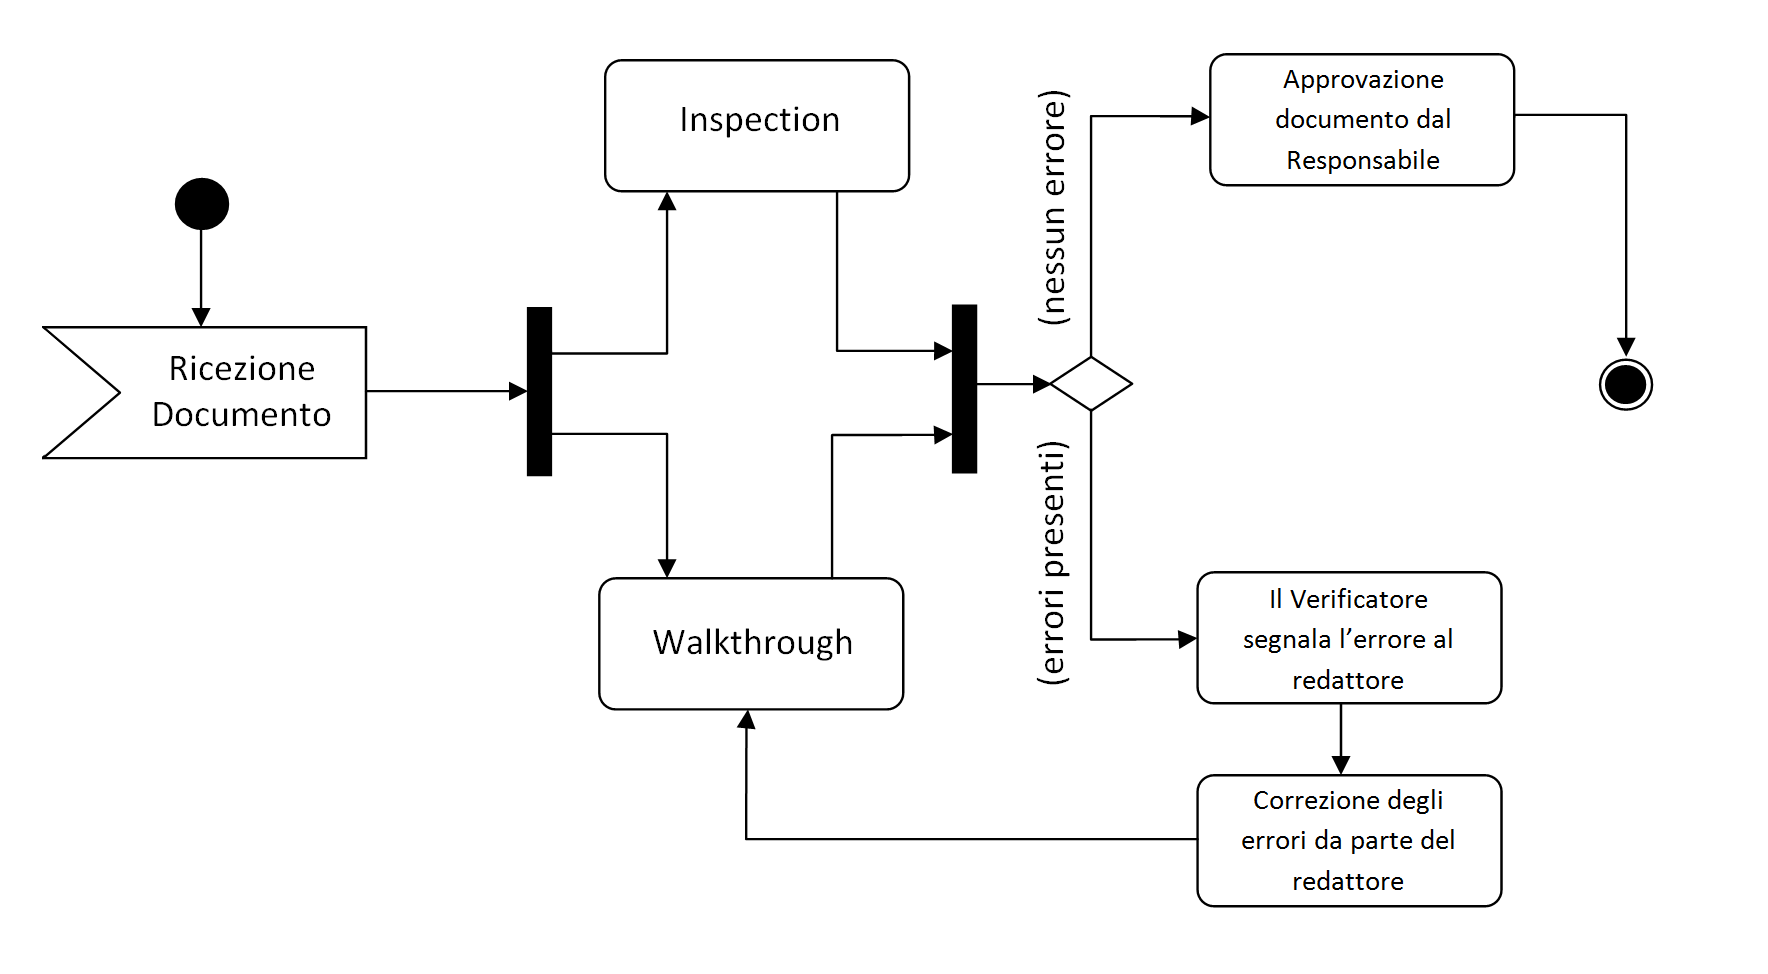
\includegraphics[scale=.45]{img/schema_RR.png}
	\caption{Verifica dei documenti}
\end{figure}

\subsubsection{Progettazione Architetturale}
Il processo di verifica in fase di Progettazione consisterà nel verificare che tutti i requisiti descritti durante la fase di Analisi dei Requisiti siano tracciabili nei componenti individuati e viceversa che ogni componente soddisfi o sia associato ad almeno un requisito. Qualora dalla verifica sorgano incongruenze o mancanze, queste verranno segnalate tramite ticket e successivamente risolte. Nello svolgere questa attività il gruppo di lavoro dovrà porsi come obiettivo il conseguimento delle seguenti proprietà:

\begin{itemize}
	\item \textbf{Semplicità}: i componenti devono contenere solo quello che è necessario al loro funzionamento;
	\item \textbf{Coesione}: misura quanto sono collegati tra di loro le componenti di un modulo. Se i metodi di una classe svolgono compiti simili, il grado di coesione di tale classe è alto. L'obiettivo sarà quello di massimizzare questo aspetto;
	\item \textbf{Incapsulamento}: ll funzionamento interno di una classe viene nascosto all'esterno, proteggendo così gli utenti di quella classe da eventuali modifiche;
	\item \textbf{Accoppiamento}: indica quanto una componente fa affidamento sull'altra, dipendendo da essa. Un basso grado di accoppiamento favorisce la manutenibilità del software.
\end{itemize}
Gli obiettivi di qualità vengono descritti nel capitolo 3. il lavoro del  \ruoloVerificatore\ è quello di effettuare una verifica incrociata tra i requisiti riportati nel documento\textit{ AnalisiDeiRequisiti\_v3.0.pdf} e le componenti descritte nel documento \textit{SpecificaTecnica\_v3.0.pdf}, accertandosi  i requisiti utente siano soddisfatti  dalle componenti architetturali prodotte durante la progettazione ad alto livello e dai metodi e dagli attributi prodotti nella progettazione di dettaglio.
Le attività di tracciamento, controllo diagrammi UML e verifica della progettazione vengono eseguite in parallelo assicurando il soddisfacimento delle quattro proprietà descritte sopra. Inoltre, i \textit{Verificatori} devono controllare che:

\begin{itemize}
	\item non vi sia eccessiva complessità nelle componenti del sistema;
	\item ciascuna parte individuata non sia ulteriormente divisibile;
	\item i pattern utilizzati siano descritti e motivati, specificando i vantaggi e le implicazioni derivanti dalla loro adozione;
	\item i pattern siano usati correttamente nell'architettura del sistema;
\end{itemize}

I diagrammi UML devono essere conformi a quanto segue:
\begin{itemize}
	\item essere conformi allo standard 2.0;
	\item non possedere associazioni scorrette;
	\item avere una complessità non eccessiva: la complessità è troppo elevata se è possibile individuare dei gruppi logici indipendenti in uno stesso diagramma. Ciò è causa di errori, diminuisce la comprensibilità e riduce il tempo di vita del diagramma stesso, in quanto una delle componenti rappresentate potrebbe essere soggetta a cambiamenti;
	\item non possedere relazioni di dipendenza scorrette;
	\item le classi devono essere posizionate correttamente (al posto giusto e nel package giusto).
\end{itemize}

\begin{figure}[h!]
	\centering
	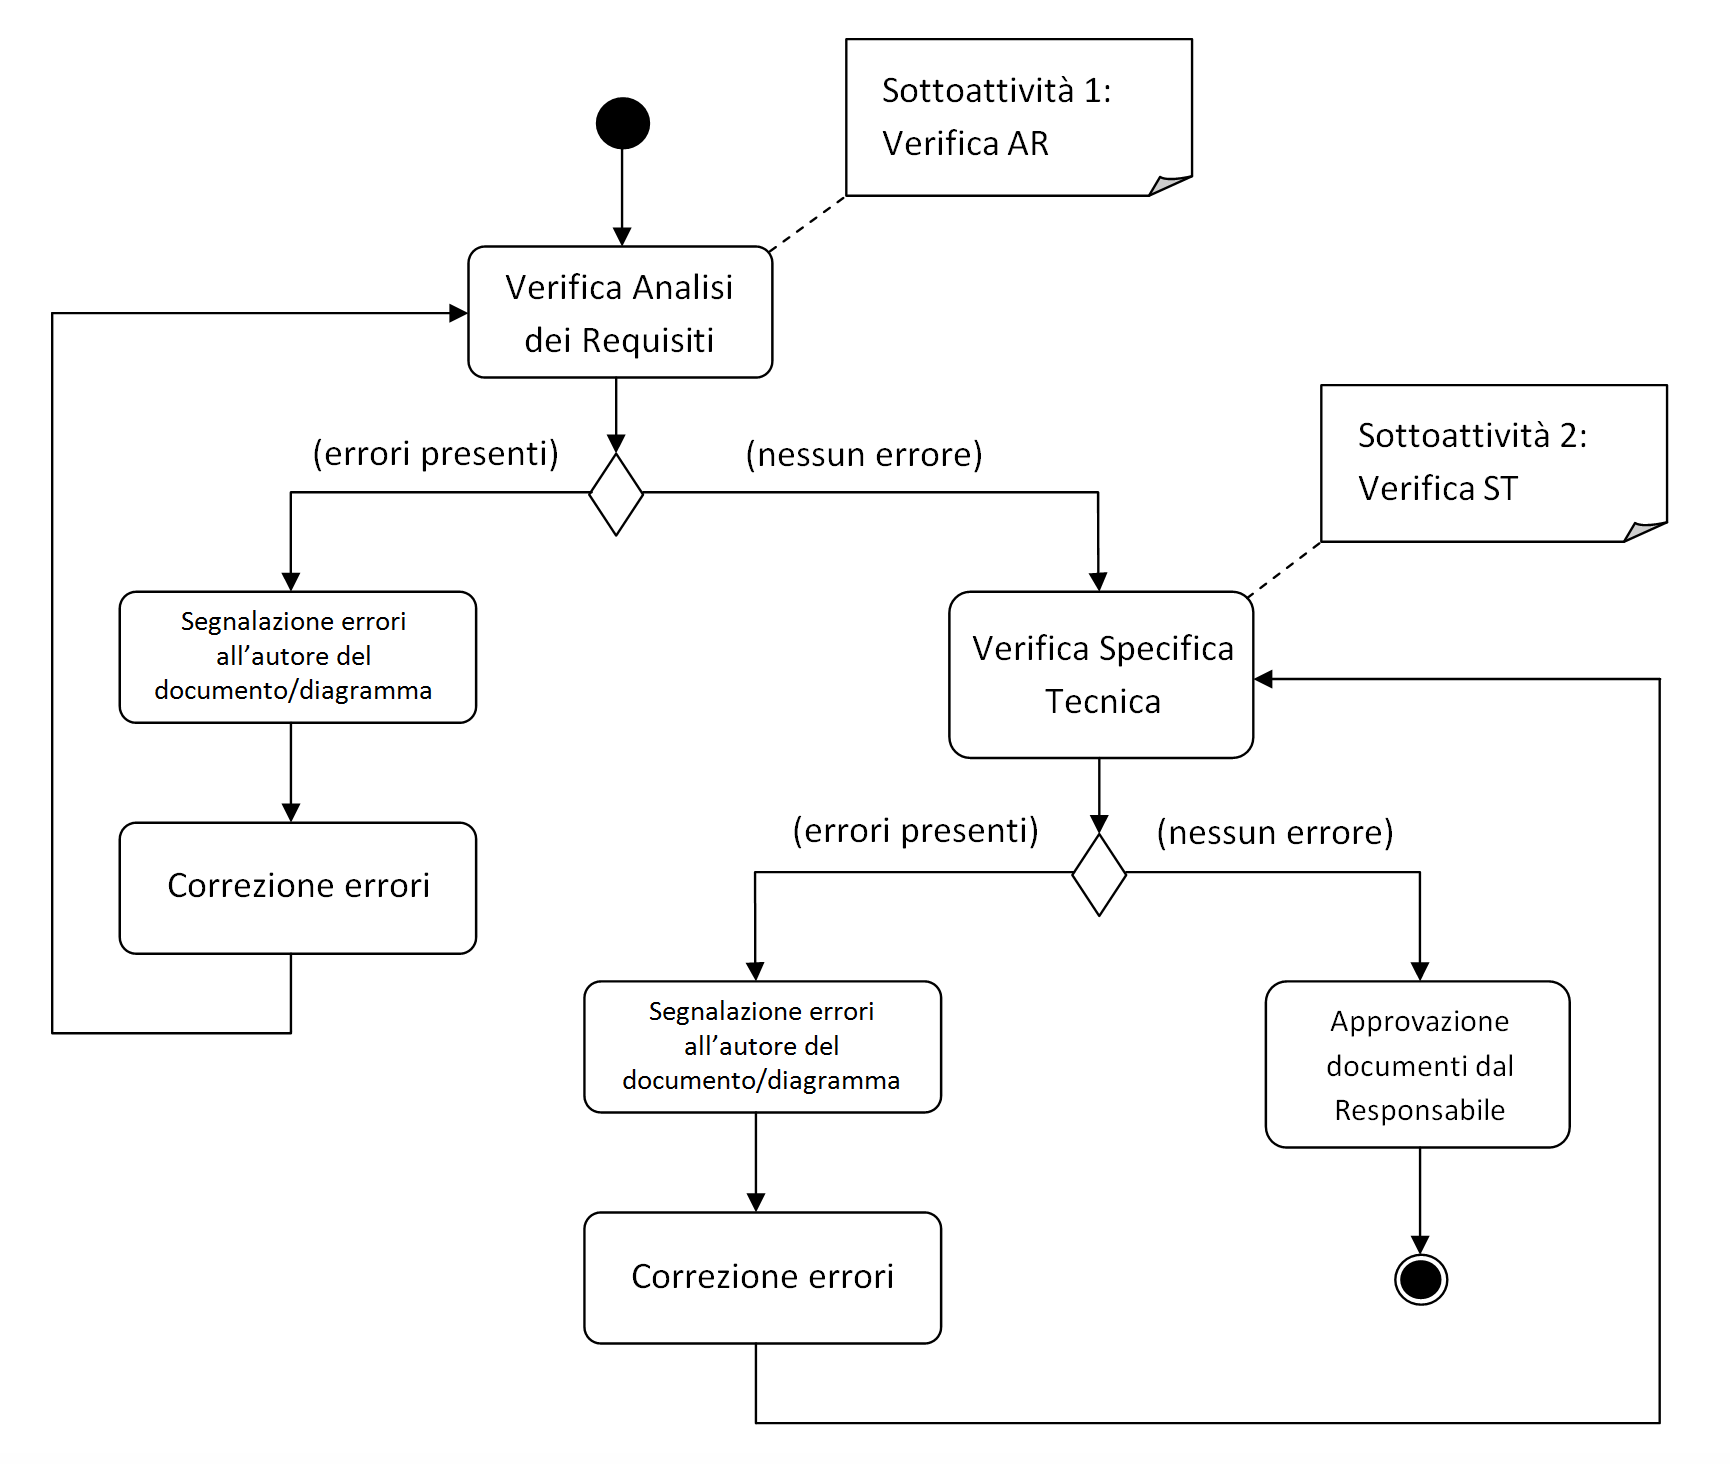
\includegraphics[scale=.45]{img/schema_RP.png}
	\caption{Verifica della progettazione}
\end{figure}

\begin{figure}[h!]
	\centering
	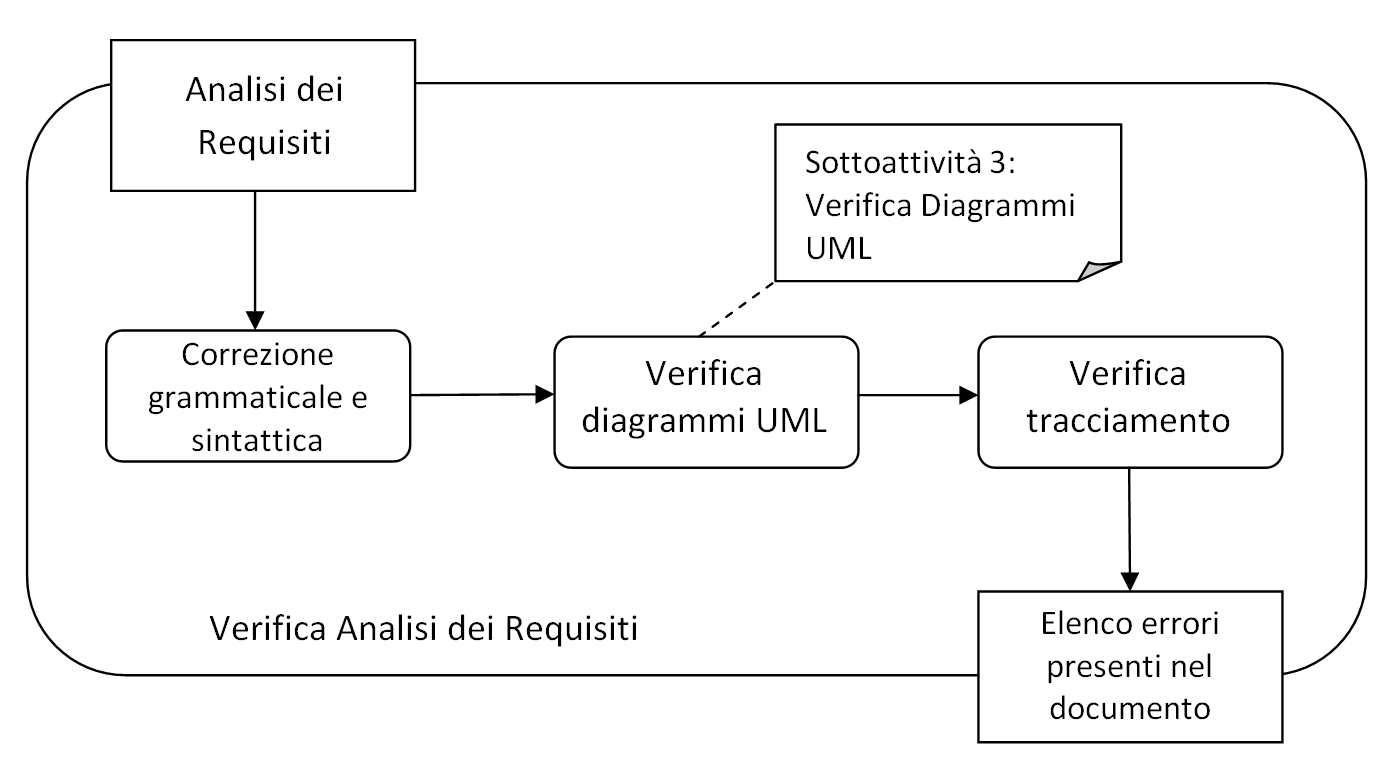
\includegraphics[scale=.45]{img/schema_AR.png}
	\caption{Sottoattività 1: Verifica dell'Analisi dei Requisiti}
\end{figure}

\begin{figure}[h!]
	\centering
	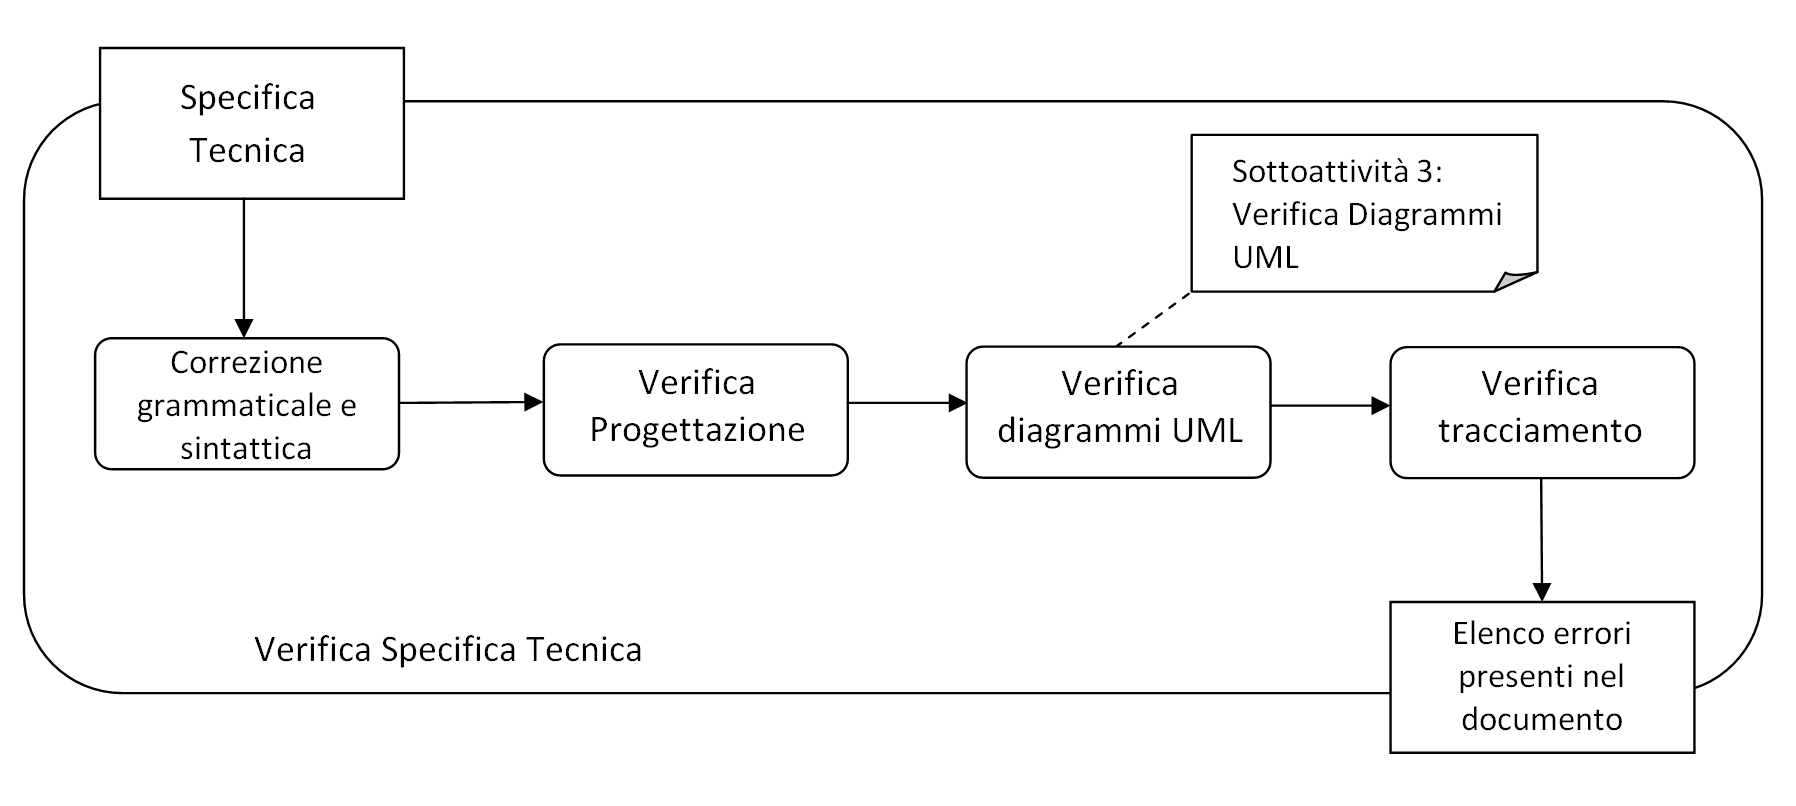
\includegraphics[scale=.45]{img/schema_ST.png}
	\caption{Sottoattività 2: Verifica della Specifica Tecnica}
\end{figure}

\begin{figure}[h!]
	\centering
	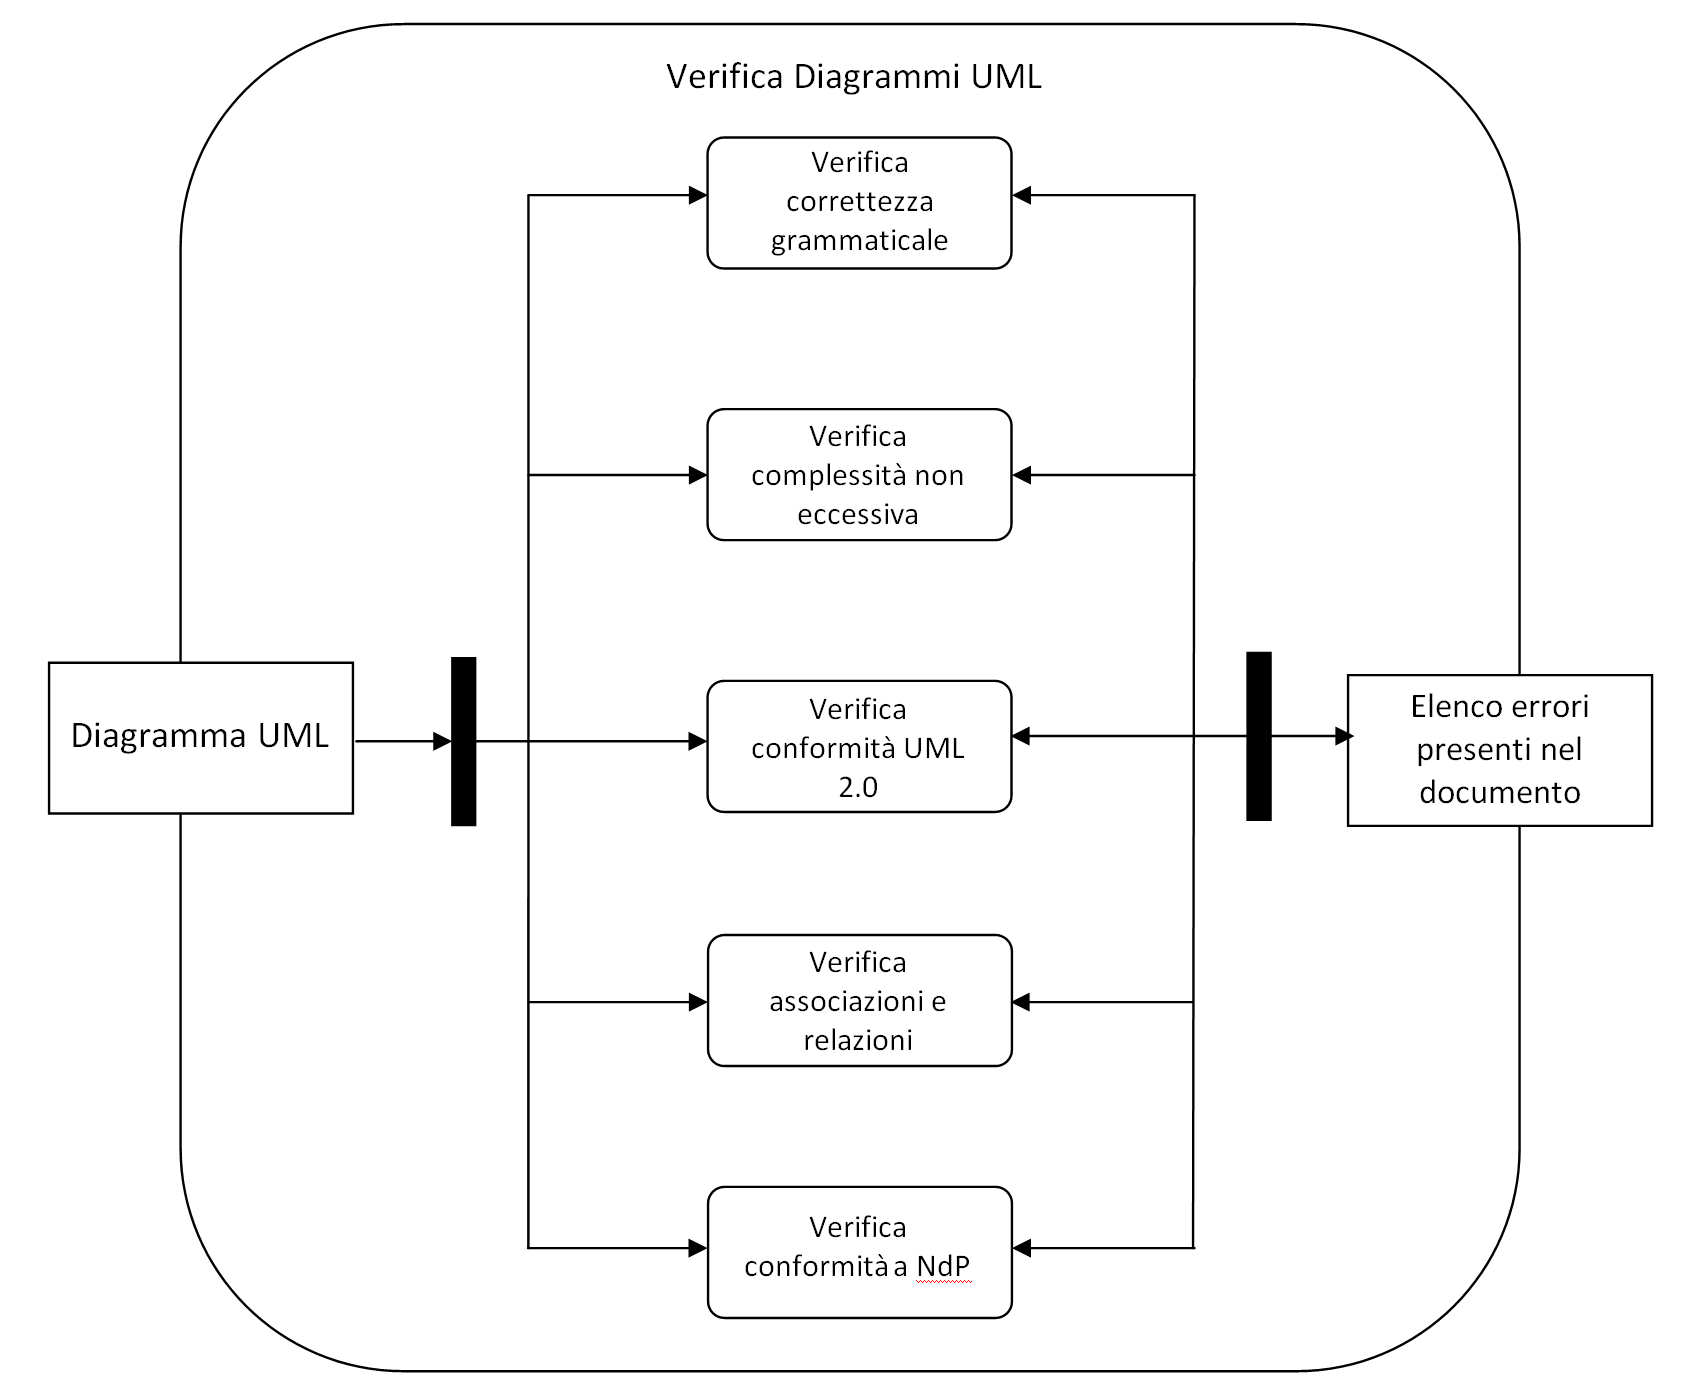
\includegraphics[scale=.45]{img/schema_UML.png}
	\caption{Sottoattività 3: Verifica dei diagrammi UML}
\end{figure}

\subsubsection{Programmazione di dettaglio e codifica}
La verifica in questa fase verrà effettuata da parte
dei programmatori stessi utilizzando appositi e specifici strumenti di verifica automatizzata del codice. La presenza di errori verrà segnalata da un apposito ticket che verrà preso in carico dai programmatori e chiuso una volta risolto il problema.
Devono essere effettuati test di unità, scritti anch'essi dai programmatori, per verificare che il comportamento del codice che hanno scritto corrisponda a quanto ci si aspetta. Un test su un'unità è composto da:

\begin{itemize}
	\item[-] l'oggetto su cui viene eseguito il test;
	\item[-] la strategia utilizzata per effettuare la prova;
	\item[-] il piano di esecuzione del test stesso, che comprende gli ingressi del test e deve prevederne le uscite attese.
\end{itemize}
Perchè sia possibile individuare il maggior numero di errori possibile è necessario che i test vengano pianificati assicurando:

\begin{itemize}
	\item \textbf{Statement Coverage}: il test deve coprire tutte le linee di codice del modulo in esame;
	\item \textbf{Branch Coverage}: il test deve coprire tutti i rami del flusso di controllo almeno una volta.
\end{itemize}
Questi test apparterranno alla categoria white box: eseguiti cioè conoscendo in dettaglio il codice sorgente delle singole unita` e analizzando come, a partire dagli input, sono prodotti gli output.
In questo modo si garantisce la correttezza logica di ogni metodo.
I verificatori dovranno poi eseguire un'attività di inspection (vedi sezione 2.7.2) su quanto scritto dai programmatori secondo la seguente lista di controllo:

\begin{itemize}
	\item[-] le variabili globali non sono ammesse;
	\item[-] le variabili vanno inizializzate al momento della dichiarazione;
	\item[-] non sono ammesse variabili e metodi non utilizzati;
	\item[-] minimizzare, se non eliminare, la presenza di alert$_G$ o altre forme di warning$_G$.
	\item[-] l'uso del break$_G$ non `e ammesso se non all'interno dei costrutti switch$_G$ , che devono comunque essere presenti il più esiguamente possibile nel codice in quanto aumentano la complessità ciclomatica di 1 per ogni ramo case;
	\item[-] le variabili che controllano l'uscita dai cicli non devono poter essere modificate dall'esterno del ciclo;
	\item[-] deve essere favorita la lazy evaluation$_G$ delle condizioni booleane;
	\item[-] il codice deve essere il più possibile comprensibile; qualora risulti di difficile comprensione il programmatore deve inserire dei commenti. I commenti non vanno tuttavia inseriti per descrivere righe il cui significato è ovvio;
	\item[-] i commenti al codice devono essere scritti in italiano;
	\item[-] l'indentazione deve essere consistente e favorire la lettura del codice.
\end{itemize}

Vanno infine garantite le caratteristiche di qualità descritte dallo standard ISO/IEC 91264 e riportate in nella sezione 3.2 del presente documento e il rispetto dei valori per le metriche stabiliti nella sezione 2.7.3.

\begin{figure}[h!]
	\centering
	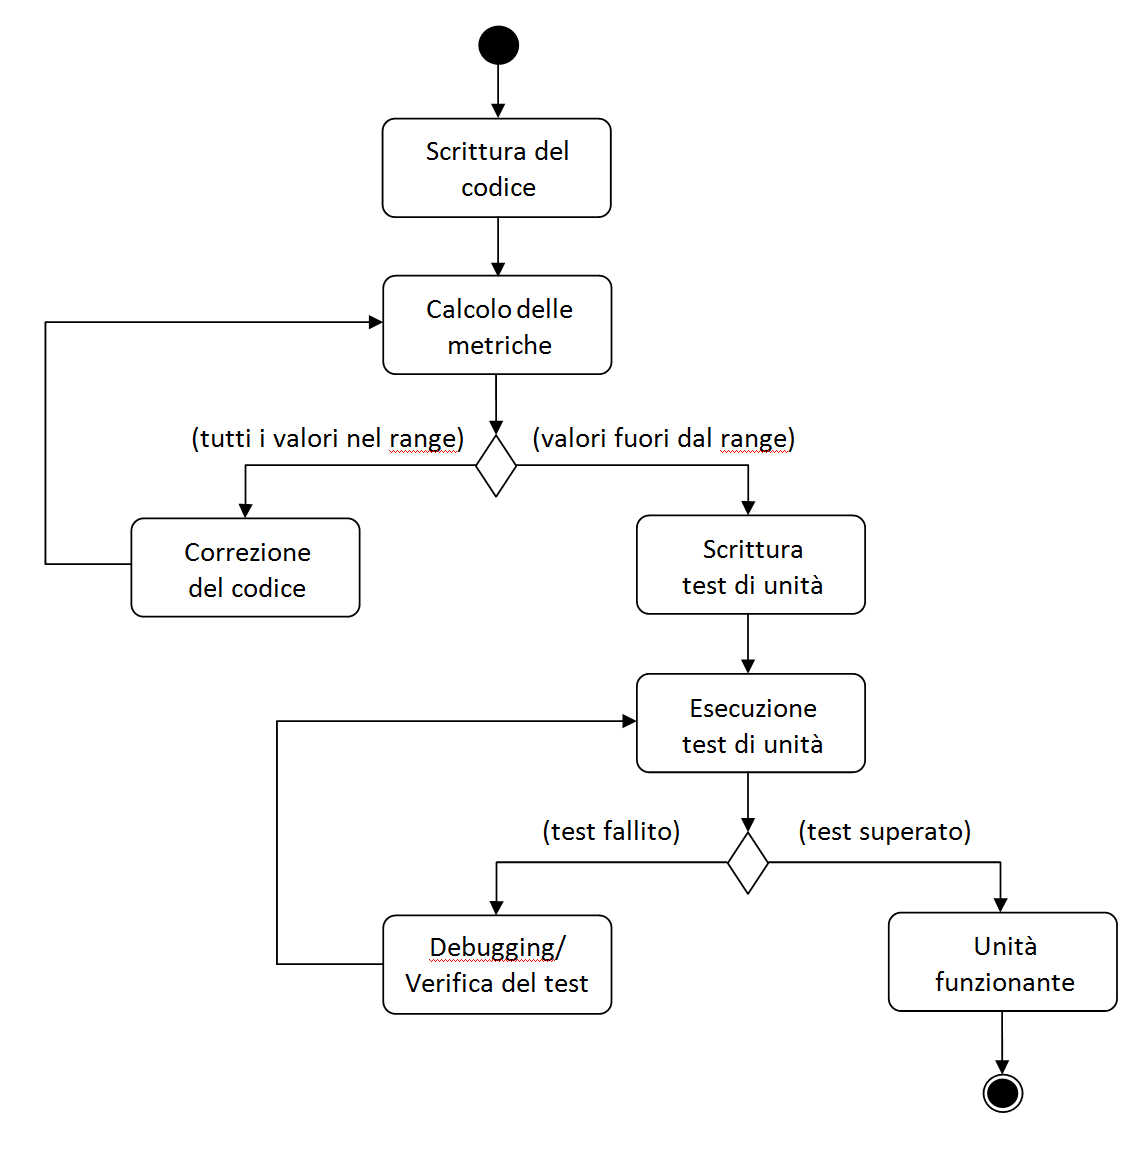
\includegraphics[scale=.5]{img/schema_Test.png}
	\caption{Verifica della codifica}
\end{figure}

\subsubsection{Test e Validazione}
Il team \gruppo\ si impegna a garantire il corretto funzionamento del prodotto Premi e a fornire al collaudo una versione funzionante e possibilmente completa del prodotto. Nel caso in cui vengano riscontrati malfunzionamenti o discrepanze tra le caratteristiche del prodotto e le richieste del cliente sarà cura del fornitore eliminare tali difetti, interamente a proprio carico. I test devono essere contraddistinti da un ID, devono elencare le componenti in esame e le modalità di testing. Nell'appendice A vengono elencati i test svolti dal gruppo per lo sviluppo dell'applicazione Premi.\\ \\
Quando tutte le componenti sono state testate e integrate si procede con il test di sistema, che controlla che il prodotto svolga correttamente i suoi compiti e rispetti i requisiti fissati in sede di analisi. Il controllo di sistema si divide in due categorie:

\begin{itemize}
	\item \textbf{Alfa-test}: consiste nell'utilizzo del software, effettuato all'interno del gruppo, andando a testare tutte le funzionalità e inserendo istruzioni di controllo a tempo di esecuzione, segnalando eventuali malfunzionamenti;
	\item \textbf{Beta-test}: consiste in un utilizzo normale del prodotto, effettuato possibilmente da membri estranei al team di sviluppo, alla ricerca degli ultimi problemi residui.
\end{itemize}

\subsection{Responsabilità}
Per garantire che il processo di verifica sia efficace e sistematico vengono attribuite delle responsabilità ad ogni specifico ruolo del progetto. I ruoli che detengono le responsabilità del processo di verifica sono il \ruoloResponsabile\ ed i {\textit{Verificatori}}. La suddivisione dei compiti e le modalità di attuazione degli stessi sono definiti nel documento\textit{NormeDiProgetto\_v3.0.pdf}.

\subsection{Risorse}
Per assicurare che gli obiettivi qualitativi vengano raggiunti è necessario l'utilizzo di risorse sia umane che tecnologiche. Coloro che detengono la responsabilità maggiore per l'attività di verifica e validazione sono il \ruoloResponsabile\ e il \ruoloVerificatore. Per una dettagliata descrizione dei ruoli e delle loro responsabilità fare riferimento alle \textit{NormeDiProgetto_v3.0.pdf}. Per risorse tecniche e tecnologiche sono da intendersi tutti gli strumenti software e hardware che il gruppo intende utilizzare per attuare le attività di verifica su processi e prodotti.

\subsection{Strumenti, Tecniche e Metodi}
\subsubsection{Strumenti}
Per lo svolgimento del processo di verifica faremo uso dei seguenti strumenti:
\begin{itemize}
	\item \textbf{Correttore automatico di TeXMaker$_G$}: come segnalato nelle \textit{NormeDiProgetto\_v3.0.pdf} per la scrittura di documenti si è scelto di utilizzare l'ambiente grafico TeXMaker$_G$. Tale strumento integra i dizionari di OpenOffice.org e segnala i potenziali
	errori ortografici presenti nel testo;

	\item \textbf{404TrackerDB}: Strumento software realizzato dal gruppo \gruppo\ che contiene ed associa:
	\begin{itemize}
		\item Requisiti individuati durante l'analisi;
		\item Fonti di requisiti individuate, inclusi anche i casi d'uso.
	\end{itemize}
	Permette inoltre di esportare automaticamente:
	\begin{itemize}
		\item Codice \LaTeX\ per la descrizione dei casi d'uso;
		\item Tabella in \LaTeX\ per il tracciamento fonti-requisiti.
	\end{itemize}

	\item Strumenti W3C$_G$ (\href{www.w3.org}{www.w3.org}) per la validazione:
	    \begin{itemize}
	    	\item \textbf{validatore HTML5$_G$} (\href{http://validator.w3.org}{http://validator.w3.org});
	    	\item \textbf{validatore CSS$_G$}
	    	(\href{http://jigsaw.w3.org/css-validator/}{http://jigsaw.w3.org/css-validator/}).
	    \end{itemize}
	
	\item Strumenti per debugging$_G$ HTML$_G$, CSS$_G$ e JavaScript$_G$ messi a disposizione dai vari browser$_G$:
	    \begin{itemize}
	    	\item \textbf{Chrome Developer Tools} (\href{https://developers.google.com/chrome-developer-tools}
	    	{https://developers.google.com/chrome-developer-tools});
	    	\item \textbf{Firebug}
	    	(\href{http://getfirebug.com/}{http://getfirebug.com/}).
	    \end{itemize}
	\item \textbf{JSLint} Ambiente di test (\href{http://www.junit.org}{http://www.junit.org}): tool per la validazione di codice JavaScript$_G$;
	\item \textbf{Plato} (\href{https://github.com/jsoverson/plato}{https://github.com/jsoverson/plato}): visualizzatore del codice sorgente, strumento per l'analisi statica e calcolo della complessità.
	\item \textbf{BrowserStack} (\href{http://www.browserstack.com/}{http://www.browserstack.com/}):  per eseguire il test comparato sui vari browser$_G$;
	\item \textbf{WebStorm} (\href{https://www.jetbrains.com/webstorm/}{https://www.jetbrains.com/webstorm/}): IDE JavaScript$_G$ scelto come ambiente di sviluppo.
\end{itemize}

\subsubsection{Tecniche di Analisi}
\textbf{Anamilisi Statica}:\medskip \\ 
Consiste nell'analisi della documentazione e dei prodotti software senza effettuare l'esecuzione. Viene svolta mediante due tecniche complementari:
\begin{itemize}
	\item \textbf{Walkthrough}:
	È una tecnica che viene utilizzata soprattutto nelle prime fasi del progetto, quando ancora non è stata maturata una adeguata esperienza da parte dei membri del gruppo, che permetta di attuare una verifica più mirata e precisa. Consiste nella rilettura completa e metodica da
	parte dell'autore stesso o da parte del \ruoloVerificatore\ allo scopo di trovare errori. Con l'utilizzo di questa tecnica, il Verificatore sarà in grado di stilare una lista di controllo con gli errori più frequenti in modo da favorire il miglioramento di tale attività nelle fasi future. Questa è un'attività onerosa e collaborativa che richiede l'intervento di più persone per essere efficace ed efficiente. Segue una fase di discussione con la finalità di esaminare i difetti riscontrati e di proporre le dovute correzioni. L'ultima fase consiste nel correggere gli errori rilevati;
	\item \textbf{Inspection}:
	Questa tecnica consiste nell'analisi di alcune parti del documento o del codice alla ricerca di errori solo in parti ritenute critiche in base all'esperienza derivata dalle revisioni precedenti. La lista di controllo o checklist, che deve essere seguita per svolgere efficacemente questo processo, deve essere redatta anticipatamente ed è frutto del lavoro svolto dai verificatori con la tecnica di walkthrough. L'Inspection è da preferire al Walkthrough, poiché  non necessità della lettura integrale dei documenti in oggetto, ma richiede un sufficiente livello di dettaglio nella lista di controllo.	    
\end{itemize}
\textbf{Metodi di Analisi Statica}:
\begin{itemize}
	\item \textbf{Analisi del flusso di controllo}: si controlla che il codice sia correttamente strutturato e che segua il flusso aspettato, che non vi siano parti del programma che possano non terminare e che non esistano porzioni di codice non raggiungibile;
	\item \textbf{Analisi del flusso dei dati}: si accerta che il software non acceda mai a variabili non inizializzate o non modifichi più volte di seguito una variabile senza leggerne il valore tra una modifica e l'altra;
	\item \textbf{Analisi del flusso di informazione}: si verifica che le uniche dipendenze tra gli input e gli output di ogni unità di codice o di più unità siano quelle previste in fase di progettazione.
\end{itemize}
\textbf{Analisi Dinamica}:\medskip \\
Consiste nella verifica dei componenti del software o del sistema in generale e richiede l'esecuzione del programma per eseguire il test.
Perché tale attività sia utile e generi risultati attendibili è necessario che i test effettuati siano ripetibili: cioè dati uno stesso input e uno stesso ambiente di esecuzione deve fornire gli stessi risultati quando vengono effettuate più prove. Questi risultati saranno utili solo se porteranno alla luce errori permettendo di correggerli, nel caso non vengano riscontrate anomalie, ciò non costituisce una prova dell'assenza di errori.
\\ \\ \textbf{Metodi di Analisi Dinamica}:
\begin{itemize}
	\item \textbf{Test di unità}:
	Viene verificata ogni unità software che deve soddisfare i requisiti per essa richiesti ed è necessario testare tutte le possibili esecuzioni del codice che la compongono. Per unità si intende la più piccola quantità di software che è utile verificare singolarmente e che viene prodotta da un singolo \ruoloProgrammatore;
	\item \textbf{Test di integrazione}:
	I moduli che hanno superato il test di unità possono
	venire integrati tra di loro. Il test di integrazione ha lo scopo di individuare errori residui nella realizzazione dei moduli e problemi nell'integrazione con altre componenti fornite da terze parti che non si conoscono a fondo;
	\item \textbf{Test di sistema e collaudo}:
	Serve a verificare il completo soddisfacimento dei requisiti software stabiliti in fase di Analisi. Consiste nella validazione del prodotto software nel momento in cui vengono aggiunti tutti i componenti. Il test potrà riguardare, in una fase iniziale, solamente alcune delle componenti del prodotto finale, per poi interessare il sistema nella sua interezza;
	\item \textbf{Test di regressione}:
	Consiste nell'eseguire nuovamente i test di unità e di integrazione su componenti software alle quali sono stati apportati cambiamenti. Serve a  controllare che le modifiche apportate non provochino malfunzionamenti alla componente stessa o ad altre che dipendono da essa;
	\item \textbf{Test di accettazione}:
	È il test di collaudo del prodotto software che viene eseguito in presenza del Committente. Se questa fase finale di test viene superata positivamente si può procedere al rilascio ufficiale del prodotto sviluppato.
\end{itemize}
\newpage
\subsubsection{Misure e Metriche}
Le misure e le metriche che il team adotterà si ispireranno alle indicazioni dello standard ISO/IEC$_G$-14598. Tale norma descrive il processo di valutazione della qualità del software. Vengono di seguito descritte le metriche sulle quali \gruppo\ intende basarsi nei processi di verifica, sia in fase di progettazione che di codifica, che potranno essere integrate e stabilite con maggiore precisione durante l'avanzamento del progetto.

Essendo la natura delle metriche molto variabile, vi possono essere due tipologie di range:

\begin{itemize}
\item \textbf{Accettazione}: valori da rispettare affinché il prodotto possa essere accettato;
\item \textbf{Ottimale}: valori entro cui dovrebbe collocarsi la misurazione. Tale range non è vincolante, ma fortemente consigliato.
\end{itemize}

\begin{itemize}
    \item \textbf{Complessità ciclomatica}:
    La complessità ciclomatica di un programma è il
    numero di cammini linearmente indipendenti attraverso il codice sorgente. Per esempio, se il codice sorgente non contiene IF o FOR, allora il livello di complessità sarà 1, poiché esiste un solo 
    cammino, se è presente un IF la complessità diventa di 2. Un programma si può quindi rappresentare come un albero nel quale i nodi sono i blocchi del programma e gli archi sono il passaggio del controllo da un blocco all'altro. La complessità è quindi definita come:
    \begin{center}
    	\textit{C = e - n + 2p}
    \end{center}
    dove e è il numero di archi, n il numero di nodi e p il numero delle componenti connesse.  Verrà adottata la seguente tabella di riferimento per la complessità: 
    \begin{figure}[h!]
    	\centering
    	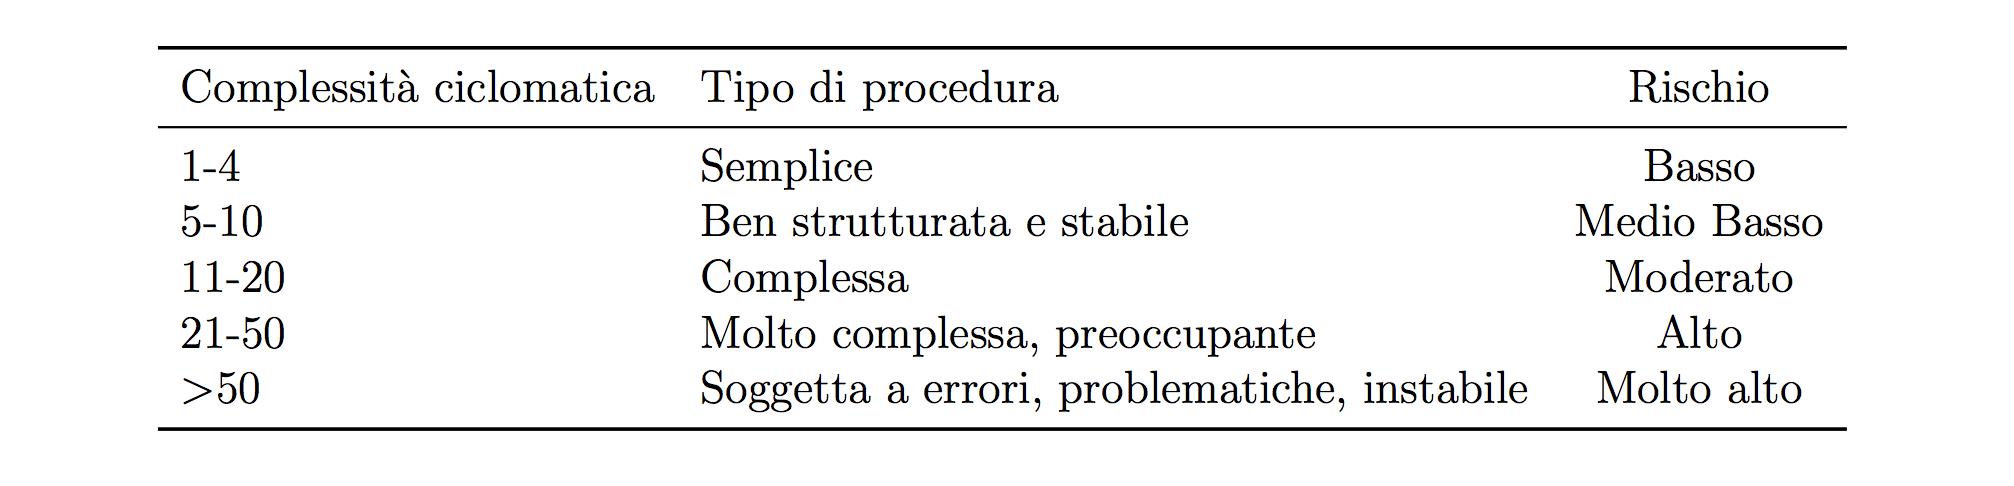
\includegraphics[scale=.45]{img/tabella_CC.png}
    	\caption{Stima della Complessità Ciclomatica}
    \end{figure} \\
    
    \textbf{Parametri utilizzati}:
    		\begin{itemize}
    			\item Range-accettazione: [1 − 20];
    			\item Range-ottimale: [1 − 10].
    		\end{itemize}
    		Il valore 10 come massimo di complessità ciclomatica fu raccomandato da T. J. McCabe, l'inventore di tale metrica.

	\item \textbf{Misure nella progettazione}:
	\begin{itemize}
		\item \textbf{Complessità di flusso}: 
		misura la quantità di informazioni in entrata ed uscita da una funzione (fan in e fan out). Fan-in è una misura del numero di metodi che invocano una determinata procedura. Un alto valore per fan-in significa che cambiamenti a quella procedura potrebbero avere effetti a catena sulle altre. Fan-out indica quanto una procedura ne richiama delle altre, dando una valutazione del grado di dipendenza di quella procedura dalle altre; Il valore è calcolato come: 
		\begin{center}
					(lunghezza funzione)$^2$ × Fan-In × Fan-Out
		\end{center}
		\item \textbf{Livelli di annidamento}: Rappresenta il numero di livelli di annidamento dei metodi, cioè l'inserimento di una struttura di controllo all'interno di un'altra. Un valore elevato di tale indice implica un'alta complessità ed un basso livello di astrazione del codice. \\
		
		\textbf{Parametri utilizzati}:
		\begin{itemize}
			\item Range-accettazione: [1 − 6];
			\item Range-ottimale: [1 − 3].
		\end{itemize} \\ \bigskip
		
		\item \textbf{Profondità di annidamento dei costrutti condizionali}: costrutti IF profondamente annidati sono più soggetti a errori e risultano più difficili da comprendere e da correggere. \\
		
		\textbf{Parametri utilizzati}:
		\begin{itemize}
			\item Range-accettazione: [0 − 3];
			\item Range-ottimale: [0 − 1].
		\end{itemize} \\ \bigskip
		
	\end{itemize}
	\item \textbf{Misure sul codice}:
	\begin{itemize}

		\item \textbf{TLOC (Total Lines Of Code)}: indice della lunghezza complessiva del codice, misura la dimensione del prodotto in termini di numero di linee di codice, al netto delle linee vuote o commentate.
		
		\item \textbf{MLOC (Method Lines Of Code)}: numero di linee di codice di un metodo, al netto delle linee vuote o commentate; Generalmente, maggiore è la dimensione di un metodo o componente, maggiore è la probabilità che esso contenga degli errori;
		
		\item \textbf{MIL (Medium Identificators Length)}: misura la lunghezza media degli identificatori (variabili, classi, metodi, etc.). Una lunghezza media elevata è indice di un elevato grado di complessità;\\
	
		Anche se si ritiene ragionevole porsi l'obiettivo di mantenere la lunghezza dei moduli al di sotto delle 400 righe per agevolarne la manutenibilità, le metriche dimensionali,  riguardanti cioè il numero di linee di codice, non devono essere viste troppo rigidamente. Nella maggior parte dei casi la lunghezza non dovrebbe comunque superare le poche decine di righe. \\
		
		\textbf{Parametri utilizzati}:
		\begin{itemize}
			\item Range-accettazione: [0 − 400];
			\item Range-ottimale: [0 − 50].
		\end{itemize} \\ \bigskip
		
		 \item \textbf{NOF (Number Of Fields)}: è il numero totale dei campi dati per classe; \\
		
		\textbf{Parametri utilizzati}:
		\begin{itemize}
			\item Range-accettazione: [0 − 30];
			\item Range-ottimale: [5 − 20].
		\end{itemize} \\ \bigskip
		
		\item \textbf{NOP (Number Of Parameters)}: indica il numero di parametri formali nei metodi. Quando questo indice è troppo elevato, è opportuno pensare di semplificare i metodi suddividendoli in metodi più semplici. \\
		
		\textbf{Parametri utilizzati}:
		\begin{itemize}
			\item Range-accettazione: [0 − 6];
			\item Range-ottimale: [0 − 4].
		\end{itemize} \\ \bigskip

		\item \textbf{NOM (Number of Methods)}: è il numero totale di metodi in un particolare scope$_G$; \\
		
		\textbf{Parametri utilizzati}:
		\begin{itemize}
			\item Range-accettazione: [0 − 20];
			\item Range-ottimale: [0 − 7].
		\end{itemize} \\ \bigskip

		\item \textbf{PAR (Number of Parameters)}: è il numero totale di parametri in un particolare scope$_G$. \\
		
		\textbf{Parametri utilizzati}:
		\begin{itemize}
			\item Range-accettazione: [0 − 9];
			\item Range-ottimale: [0 − 4].
		\end{itemize}
	\end{itemize}
\end{itemize}
